% ************************** Thesis Chapter3 **********************************
\chapter{การดำเนินงานวิจัย}
\section{แผนการดำเนินงาน}
การออกแบบหุ่นยนต์ฮิวมานอยด์นั้น ผู้วิจัยได้มีการตั้งชื่อให้หุ่นยนต์ โดยใช้ชื่อว่า อุทัย (UTHAI)
มาจากภาษาอังกฤษคำว่า Universal Template for Humanoid Algorithm Interface
เพื่อให้สมกับเป็นหุ่นยนต์ฮิวมานอยด์ที่ใช้สำหรับงานวิจัยและพัฒนาต่อยอด

\hspace{-100pt}
\begin{ganttchart}[
		y unit title=0.5cm,
		y unit chart=0.6cm,
		vgrid={*6{draw=none}, dotted},
		hgrid,
		x unit=1.25pt,
		time slot format=isodate,
		% compress ca1lendar,
		title/.append style={shape=rectangle, fill=black!10},
		title height=1,
		bar/.append style={fill=green!90},
		bar height=.6,
		bar label font=\normalsize\color{black!50},
		group top shift=.6,
		group height=.3,
		group peaks height=.3,
	]{2017-08-01}{2018-05-20}
	\gantttitlecalendar{year,month} \\
	
	\ganttset{progress label text={},
		bar incomplete/.append style={fill=green!40},
		group/.append style={draw=black, fill=green},} % this suppresses percentage done labels
	\ganttgroup{Design}{2017-08-01}{2018-01-01} \\
	\ganttbar[progress=00, name=bg_research]{Background Research}{2017-08-01}{2017-08-31} \\
	\ganttlinkedbar[progress=00, name=cad_analysis]{CAD analysis}{2017-08-31}{2017-09-07} \\
	% \ganttlinkedbar[progress=00, name=rflr]{R fluorescence}{2015-07}{2015-09} \\
	% \ganttlinkedbar[progress=00, name=rqpcr]{R RT-qPCR}{2015-10}{2015-11} \\
	% \ganttbar[progress=50, name=case_cad]{Case CAD}{2017-08-01}{2017-08-08} \\
	% \ganttbar[progress=00, name=case_check]{Case Check}{2017-08-01}{2017-08-08} \\
	% \ganttlinkedbar[progress=00, name=kogro]{KO growth}{2015-08}{2015-09} \\
	% \ganttbar[progress=00, name=case_printing]{Case Printing}{2017-08-01}{2017-08-08} \\
	\ganttlinkedbar[progress=00, name=lower_limb_cad]{Lower Limb CAD}{2017-09-08}{2017-10-08} \\
	\ganttlinkedbar[progress=00, name=lower_cad]{Final Lower CAD}{2017-10-09}{2017-10-15} \\
	\ganttbar[progress=00, name=lower_print]{Lower 3D printing}{2017-08-01}{2017-08-08} \\
	\ganttbar[progress=00, name=upper_limb_cad]{Upper Limb CAD}{2017-08-01}{2017-08-08} \\
	\ganttbar[progress=00, name=upper_cad]{Final Upper CAD}{2017-08-01}{2017-08-08} \\
	\ganttbar[progress=00, name=upper_print]{Upper 3D printing}{2017-08-01}{2017-08-08} \\
	\ganttbar[progress=00, name=motor_assembly]{Motor assembly}{2017-08-01}{2017-08-08} \\
	\ganttbar[progress=00, name=platfom_assembly]{Platform assembly}{2017-08-01}{2017-08-08} \\
	% \ganttlinkedbar[progress=00, name=koo2]{KO O2 evolution}{2015-10}{2015-11} \\
	\ganttset{bar incomplete/.append style={fill=red!40},
		group/.append style={draw=black, fill=red},}
	\ganttgroup{Modelling}{2017-08-01}{2018-01-05} \\
	\ganttbar[progress=00, name=box_model]{BOX model}{2017-08-01}{2017-08-08} \\
	\ganttlinkedbar[progress=00, name=mesh_model]{Mesh model}{2017-08-01}{2017-08-08} \\
	\ganttlinkedbar[progress=00, name=description_pkg]{Description Package}{2017-08-01}{2017-08-08} \\
	\ganttbar[progress=00, name=gazebo_param]{Gazebo paremeters}{2017-08-01}{2017-08-08} \\
	\ganttlinkedbar[progress=00, name=gazebo_pkg]{Gazebo Package}{2017-08-01}{2017-08-08} \\
	% \ganttbar[progress=00, name=oeclone]{Clone OEs}{2016-01}{2016-03} \\
	% \ganttbar[progress=00, name=rnagrow]{Grow KOs + OEs}{2016-04}{2016-06} \\
	% \ganttlinkedbar[progress=00, name=rnaprep]{RNA library prep}{2016-07}{2016-09} \\
	% \ganttbar[progress=00, name=rnadev]{Develop analysis}{2015-06}{2015-07} \\
	% \ganttbar[progress=00, name=rnaanal]{Analyze reads}{2016-12}{2017-02} \\
	\ganttset{bar incomplete/.append style={fill=blue!40},
		group/.append style={draw=black, fill=blue},}
	\ganttgroup{Hardware Control}{2017-08-01}{2018-01-05} \\
	\ganttbar[progress=00, name=control_config]{Setting control files}{2017-08-01}{2017-08-08} \\
	\ganttlinkedbar[progress=00, name=control_pkg]{Control Package}{2017-08-01}{2017-08-08} \\
	\ganttlinkedbar[progress=00, name=setting_motor_pkg]{Setting motor Package}{2017-08-01}{2017-08-08} \\
	\ganttlinkedbar[progress=00, name=motor_driver_pkg]{Motor driver Package}{2017-08-01}{2017-08-08} \\
	\ganttlinkedbar[progress=00, name=setting_firmware]{Setting firmware}{2017-08-01}{2017-08-08} \\
	\ganttlinkedbar[progress=00, name=final_check]{Final Check}{2017-08-01}{2017-08-08} \\
	% \ganttbar[progress=00, name=chipgrow]{Grow KOs + OEs}{2016-04}{2016-06} \\
	% \ganttlinkedbar[progress=00, name=chipprep]{ChIP library prep}{2016-08}{2016-12} \\
	% \ganttbar[progress=00, name=chipdev]{Develop analysis}{2016-01}{2016-02} \\
	% \ganttbar[progress=00, name=chipanal]{Analyze reads}{2017-03}{2017-05}
	\ganttset{bar incomplete/.append style={fill=orange!40},
		group/.append style={draw=black, fill=orange},}
	\ganttgroup{Document}{2017-08-01}{2018-01-05} \\
	\ganttbar[progress=00, name=control_config]{Setting control files}{2017-08-01}{2017-08-08} \\
	  
	% misc links
	\ganttset{progress label text={}}
	%   \ganttlink[]{oeclone}{rnagrow}
	%   \ganttlink[link mid=0.082]{oeclone}{chipgrow}
	%   \ganttlink[]{rnaprep}{rnaanal}
	%   \ganttlink[link mid=0.25]{kover}{koflr}
	%   \ganttlink[link mid=0.75]{kogro}{koo2}
	%   \ganttlink[link mid=0.55]{koo2}{oeclone}
	%   \ganttlink[link mid=0.55]{rqpcr}{oeclone}
	%   \ganttlink[]{chipprep}{chipanal}
	%   \ganttlink[link mid=0.938]{rnadev}{rnaanal}
	%   \ganttlink[link mid=0.915]{chipdev}{chipanal}
\end{ganttchart}

การดำเนินงานและการออกแบบการสร้างหุ่นยนต์ฮิวมานอยด์อุทัย มีแผนการทำงานซึ่งแบ่งออกเป็น 4 ส่วนดังนี้
ส่วนแรกคือ ส่วนของฮาร์ดแวร์ที่เกี่ยวกับโครงสร้างทางกลของหุ่นยนต์ฮิวมานอยด์ เช่น ข้อต่อ ก้านต่อ ฝ่าเท้า
รวมไปถึงระบบอิเล็กทรอนิกส์ ตัวประมวลผลการควบคุม เซนเซอร์ ตัวขับเคลื่อนต่าง ๆ และส่วนที่สองคือ
ส่วนของซอฟท์แวร์ที่เกี่ยวข้องกับการติดต่อสื่อสารกันเบื้องต้น การควบคุมตัวขับเคลื่อนที่ข้อต่อ การอ่านค่าเซนเซอร์
และระบบพื้นฐานสำหรับการใช้งาน ขั้นตอนในการทำงานวิจัยครั้งนี้


\clearpage
\section{การออกแบบโครงสร้างของหุ่นยนต์}
\subsection{การเชื่อมต่อหุ่นยนต์ฮิวมานอยด์}
โครงสร้างแพลตฟอร์มหุ่นยนต์อุทัยจะประกอบไปด้วยสองขา เพื่อทำให้เกิดองศาอิสระเป็น 12 องศาอิสระ
(DOFs) ใช้ Dynamixel servos 12 ตัว มอเตอร์ Dynamixel ทั้งหมดเชื่อมต่อกันแบบ daisy chain
ข้างนึงของมอเตอร์ตัวแรกเชื่อมต่อกับแบตเตอร์รี่ 12V และอีกข้างต่อกับ USB2Dynamixel
ทั้งหมดนี้เป็นการเชื่อมต่อ Odroid เข้ากับหุ่นยนต์ ดังรูปที่ \ref{fig:odroid2dynamixel}

\begin{figure}[htbp]
    \centering
    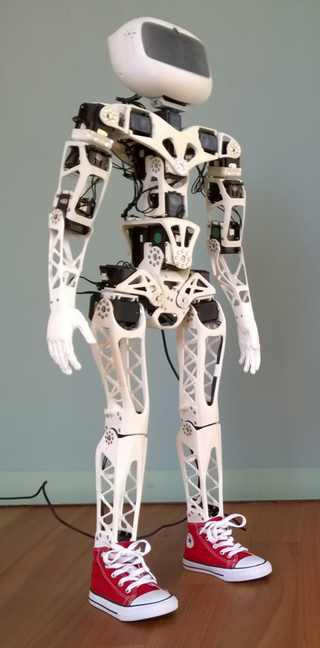
\includegraphics[width=0.3\textwidth]{chapter2/images/PoppyHumanoid1.png}
    \caption{การเชื่อมต่อระหว่าง Odroid กับ Dynamixel servos}
    \label{fig:odroid2dynamixel}
\end{figure}

หุ่นยนต์ฮิวมานอยด์อุทัยใช้เซอร์โวมอเตอร์ 12 ตัว ทำให้เกิดเป็น 12 องศาอิสระ
USB2Dynamixel ใช้เพื่อที่จะสั่งการเซอร์โวมอเตอร์ Dynamixel ผ่าน Odroid
ตำแหน่งของเซอร์โวมอเตอร์ Dynamixel EX-106+ นั้นมาจากเอนโคดเดอร์ที่อยู่ภายใน
เซนเซอร์ Gyro/Accelerometer ติดอยู่กับตัวของหุ่นยนต์ เพื่อช่วยในการทรงตัวของหุ่นยนต์
เซนเซอร์ Accelerometer จะอัพเดตค่าของตัวเองเรื่อยๆ ฟังก์ชั่นส่วนเสริมจะมาจาก ROS
และ Odroid เชื่อมต่อกับคอมพิวเตอร์ภายนอกผ่าน Wi-Fi

\subsection{อุปกรณ์ที่ใช้ในหุ่นยนต์ฮิวมานอยด์อุทัย}
\subsubsection*{Odroid}
\subsubsection*{Dynamixel servo EX-106+}
Dynamixel EX-106+ เป็นตัวขับเคลื่อนที่นิยมใช้ในปัจจุบัน โดยความสามารถของมันคือ สามารถที่จะอ่านค่าความเร็ว
แรงดันไฟฟ้า กระแสไฟฟ้า อุณหภูมิ ตำแหน่ง และแรงบิด มอเตอร์แต่ละตัวจะมีบอร์ดควบคุมของตัวเอง

\subsubsection*{USB2Dynamixel connector}
ตัวนี้เป็นอุปกรณ์สำหรับเชื่อมต่อ Odroid กับ Dynamixel โดยจะเชื่อมต่อผ่านพอร์ท USB ของ Odroid ไปยัง Dynamixel motor
ผ่านสายทั้งหมด 4 เส้น เป็นการเชื่อมต่อแบบ RS-485 
\subsubsection*{Accelerometer}
Accelerometer ที่ใช้เป็น MPU-9250 Accelerometer+Gyro+Magnito เพื่อเอาไว้ใช้หามุมเอียงของหุ่นยนต์
เทียบกับโลก
\subsubsection*{Ground contact sensor}
\subsubsection*{Wi-Fi Adapter}

\clearpage
\section{การออกแบบโปรแกรมด้วย ROS}
\subsection{Modelling}
หลังจากที่เราได้ออกแบบและโมเดลหุ่นยนต์ของเราขึ้นมาที่ใช้ CAD tools ต่างๆ เช่น AutoCAD, SolidWorks, Blender
หรืออื่นๆ ก็เพื่อที่จะนำมาใช้ในการทำ Simulation การที่เราทำ Simulation นั้นก็จะสามารถมองเห็นหุ่นยนต์
และเห็นการทำงานของหุ่นยนต์เราก่อนที่เราจะสร้างมันขึ้นมาจริงๆ หุ่นยนต์จำลองที่เราสร้างขึ้นมานั้นควรที่จะมีลักษณะให้ใกล้เคียงกับของจริงมากที่สุด
ไม่ว่าจะเป็นรูปร่าง รูปทรง น้ำหนักต่างๆ 

\subsubsection{ROS packages for robot modelling}
ROS นั้นได้ให้เครื่องมือที่ช่วยให้เราสามารถสร้าง 3D robot models ได้
ใน ROS มี meta package ที่ชื่อว่า robot\_model ซึ่งข้างในมี package ต่างๆที่ใช้สำหรับสร้าง 3D robot models
        
\paragraph*{urdf}
เป็น 1 ในหลายๆ package ที่อยู่ใน robot\_model, urdf เป็น xml ไฟล์ที่เอาไว้ใช้บอกลักษณะของหุ่นยนต์ ย่อมาจาก Unified Robot Description Format(URDF)
เราสามารถระบุ robot model, sensors และ working environment โดยใช้ URDF การบอกนั้นจะสามารถบอกเป็นเหมือน tree structure ของ link ต่างๆในตัวหุ่นยนต์ สามารถบอก rigid link เชื่อมต่อกันผ่าน joints แต่ถ้าเป็น flexible link จะไม่สามารถบอกได้โดยใช้ urdf

\subparagraph*{joint\_state\_publisher}
เครื่องมือนี้มีประโยชน์มากในการ model robot URDF เพราะมันสามารถหา joints ทุก joint ที่ไม่ใช่ fixed joints มาแสดงเป็น GUI sliders ทำให้เราสามารถเลื่อนๆหมุนๆไปมาได้ อีกทั้งยังสามารถใช้งานร่วมกับ visualize RViz

\subparagraph*{robot\_state\_publisher}
เป็นเครื่องมือที่ใช้ในการ publish 3d pose ของ link ต่างๆใน urdf การ ยublish นั้นจะใช้ ROS tf(transform) ROStf คือการหาความสัมพันธ์ระหว่าง frame ของหุ่นยนต์

\subparagraph*{xacro}
ย่อมาจาก XML Macros หรือเราสามารถเรียกอีกอย่างว่า URDF plus add-ons. ซึ่งการทำงานเหมือนกับ urdf แต่ทำให้ไฟล์ urdf สั้นกว่า อ่านง่ายกว่า และสามารถใช้เพื่อทำให้สร้างหุ่นยนต์ที่มีความซับซ้อนง่ายขึ้น เราสามารถแปลงไฟล์ xacro เป็น urdf ได้

\subsubsection{URDF}
ในส่วนนี้จะเป็นการอธิบายระบบทางกลของหุ่นยนต์ฮิวมานอยด์เป็นไฟล์ที่ใช้ร่วมกับ ROS ได้ เพื่อที่จะสามารถนำไปใช้กับ Simulation ในอนาคตได้
ในการอธิบายระบบทางกลนั้นผู้วิจัยได้ใช้ไฟล์ URDF (Universal Robotics Description Format) ซึ่งใช้ภาษาการเขียนเป็น XML ในการบอกส่วนประกอบแต่ละส่วนของหุ่นยนต์

\subsubsection*{Link}
ในไฟล์ URDF แต่ละชิ้นส่วนของหุ่นยนต์เราจะเรียกว่า link แล้วใน link จะประกอบไปด้วยส่วนย่อยๆ
3 ส่วนคือ <inertia> ที่เอาไว้บอกถึงค่าตัวแปรทางฟิสิกส์, <visual> ที่เอาไว้แสดงผลให้เราเห็น, 
<collision> ที่เอาไว้ตรวจสอบว่าหุ่นยนต์มีการชนกันกับสิ่งแวดล้อมไหม ดังตัวอย่างด้านล่างนี้

% \begin{verbatim}
% <link name="my_link">
%     <inertia>
%         <origin xyz="0 0 0.5" rpy="0 0 0"/>
%         <mass value="1"/>
%         <inertia ixx="100" ixy="0" ixz="0" iyy="100" iyz="0" izz="100"/>
%     </inertia>
%     <visual>
%         <origin xyz="0 0 0" rpy="0 0 0"/>
%         <geometry>
%             <box size="1 1 1" />
%         </geometry>
%         <material name="Cyan">
%             <color rgba="0 1.0 1.0 1.0"/>
%         </material>
%     </visual>
%     <collision>
%         <origin xyz="0 0 0" rpy="0 0 0"/>
%         <geometry>
%             <cylinder radius="1" length="0.5"/>
%         </geometry>
%     </collision>
% </link>
% \end{verbatim}

ยังมี tags อีกหลายตัวที่ใช่ในการอธิบายแต่ละชิ้นส่วนของหุ่นยนต์ แต่ตัวอย่างเป็นเพียงแค่ส่วนหนึ่งเท่านั้น
ในความเป็นจริงแล้วเราจะเขียน tags ต่างๆก็ตามที่เราต้องการ โดยใน URDF ไฟล์นั้นจะเอาไว้เก็บข้อมูลลักษณะเฉพาะของหุ่นยนต์เอาไว้
และยังสามารถใช้กับซอฟแวร์ตัวอื่นๆอีกได้
\begin{figure}[h]
	\centering
	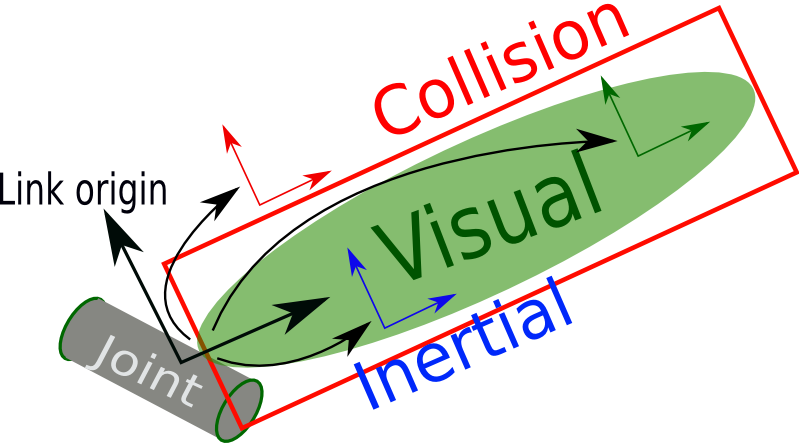
\includegraphics[width=0.45\textwidth]{chapter3/images/urdf_link.png}
	\caption{การอธิบาย link ใน URDF ไฟล์}
	\label{fig:urdf_link}
\end{figure}

\subsubsection*{Joint}
อีกส่วนที่สำคัญสำหรับการสร้างไฟล์หุ่นยนต์ด้วย URDF ก็คือ Joint tag โดย tag นี้จะอธิบายถึงความสัมพันธ์ระหว่างก้านต่อสองอัน
ส่วนนี้ไม่ได้มีเพียงแค่ทำข้อต่อให้เป็นแบบหมุนได้อย่างเดียว ยังมี Fix, Revolution, Linear และ Planar นอกเหนือจากนี้
เรายังสามารถที่จะเพิ่มองศาสูงสุดต่ำสุดของข้อต่อ รวมไปถึง dynamic properties ต่างๆ ตามที่เห็นตัวอย่างด้านล่างนี้

% \begin{verbatim}
% <joint name="my_joint" type="floating">
% <origin xyz="0 0 1" rpy="0 0 3.1416"/>
% <parent link="link1"/>
% <child link="link2"/>
% <calibration rising="0.0"/>
% <dynamics damping="0.0" friction="0.0"/>
% <limit effort="30" velocity="1.0" lower="-2.2" upper="0.7"/>
% <safety_controller k_velocity="10" k_position="15" soft_lower_limit="-2.0" soft_upper_limit="0.5"/>
% </joint>
% \end{verbatim}

เมื่อเรานำ Joint และ Link มารวมกันเราจะต้องพิจารณาว่ามีวางรูปแบบเป็นไปตามรูปที่ \ref{fig:urdf_joint}
โดยจะมีระยะระหว่างแกนของแต่ละข้อต่อกับก้านต่อ ชิ้นส่วนแรกของการสร้างไฟล์ URDF จะมีชื่อว่า base\_link
และเฟรม origin จะเป็นเฟรมอ้างอิง เมื่อเราต่อ Joint เข้ากับ Link จะเรียกก้านต่อที่เอามาติดว่า parent
โดยเฟรม origin ของข้อต่อจะอยู่จุดเดียวกับเฟรม origin ของก้านต่อ ในสถานะเดียวกันก้านต่อที่นำมาต่อจากข้อต่อ
เราจะเรียกว่า child และเฟรม origin ของก้านต่อ child จะอยู่ที่จุดเดียวกับเฟรม origin ของข้อต่อ

\begin{figure}[h]
	\centering
	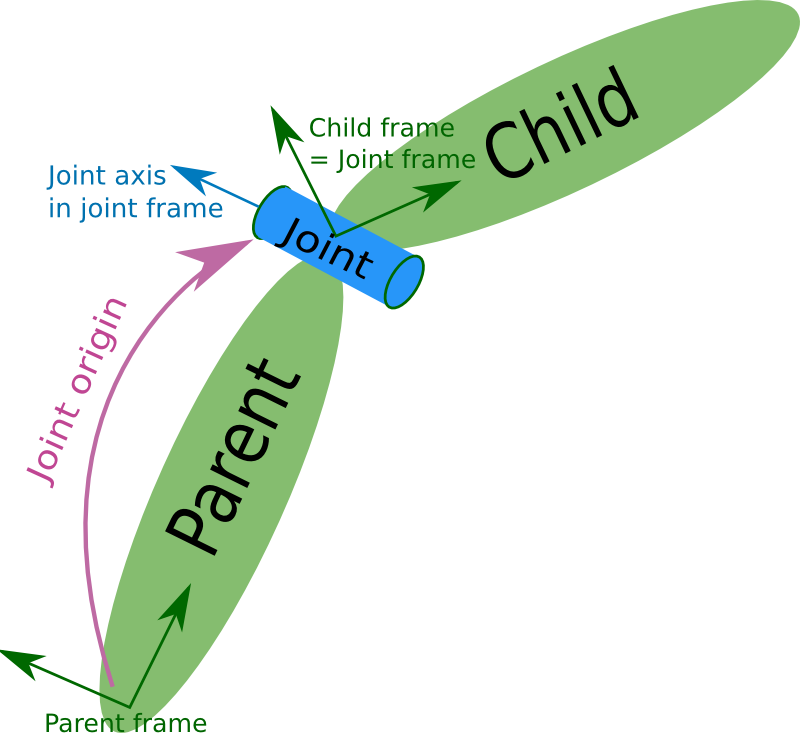
\includegraphics[width=0.45\textwidth]{chapter3/images/urdf_joint.png}
	\caption{การอธิบาย Joint ใน URDF ไฟล์}
	\label{fig:urdf_joint}
\end{figure}

\clearpage
\section{การออกแบบระบบพื้นฐาน}
\subsection*{UTHAI-Tools}
เครื่องมือสำหรับการทำงานในฮิวมานอยด์

\subsubsection*{sketch-lib}
เป็นเครื่องมือที่ใช้สำหรับเอาไว้วาดรูปเฟรมของหุ่นยนต์

\begin{figure}[htbp]
	\centering
	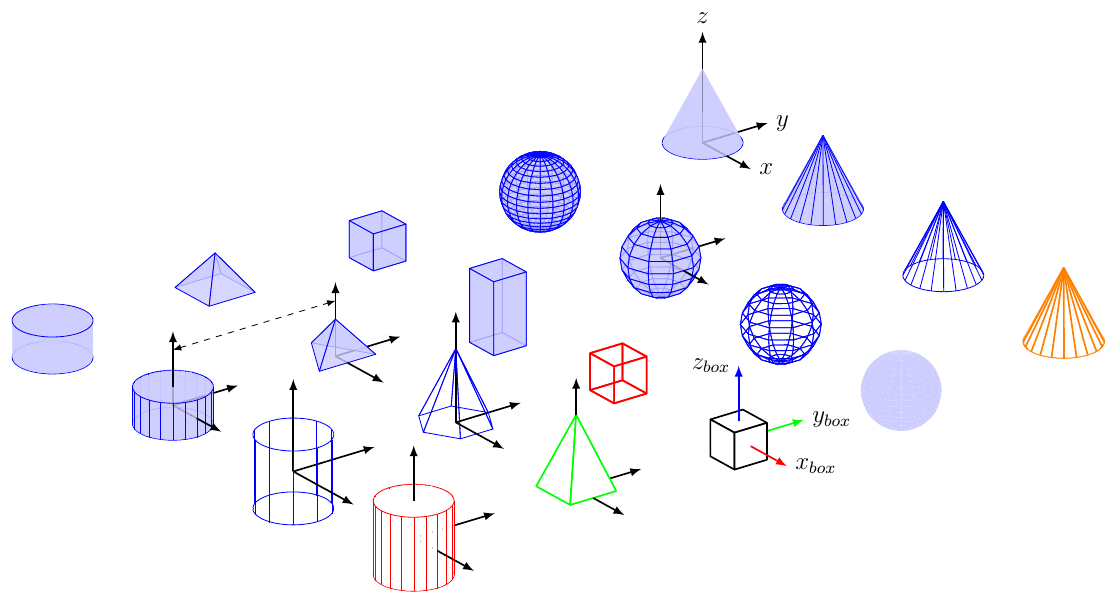
\includegraphics[width=0.7\textwidth]{chapter3/images/basic-shapes.png}
	\caption{ภาพตัวอย่างการวาดออฟเจ็คต่างๆ}
	\label{fig:basic-shapes_sk}
\end{figure}
\begin{figure}[htbp]
	\centering
	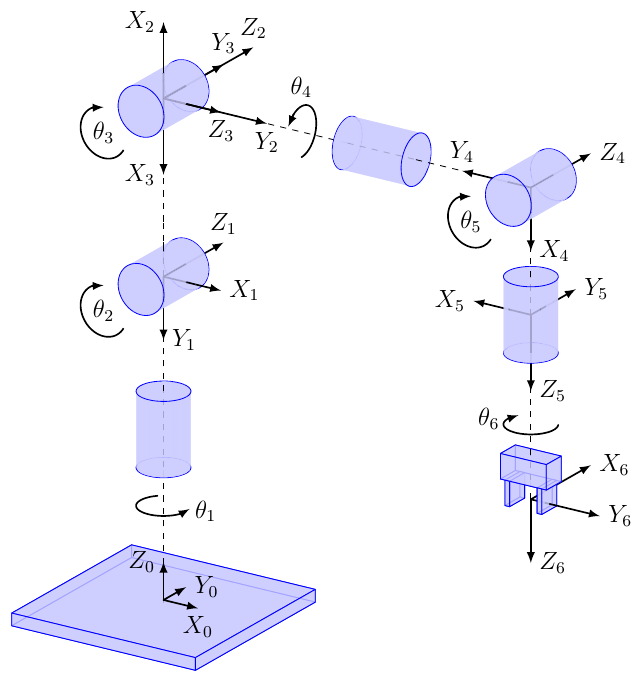
\includegraphics[width=0.5\textwidth]{chapter3/images/test_robot.png}
	\caption{ภาพตัวอย่างการวาดเฟรมของแขนกล}
	\label{fig:test-robot_sk}
\end{figure}
\begin{figure}[htbp]
	\centering
	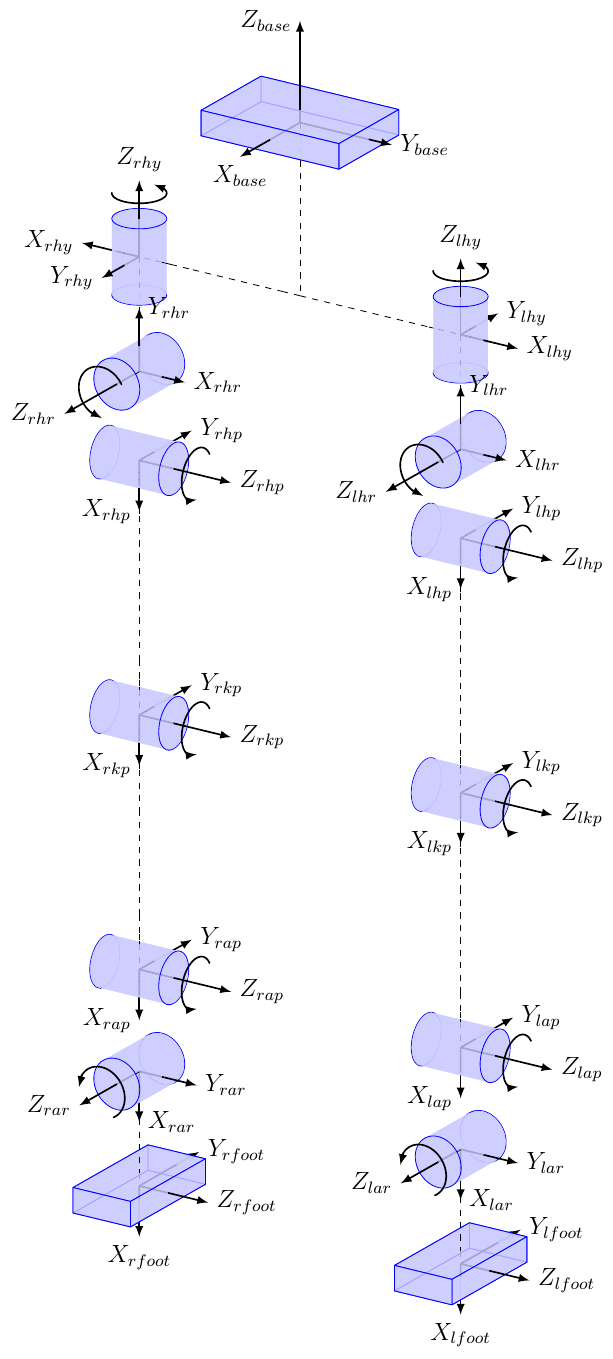
\includegraphics[width=0.4\textwidth]{chapter3/images/uthai_kinematics.png}
	\caption{ภาพตัวอย่างการวาดเฟรมของหุ่นยนต์ฮิวมานอยด์}
	\label{fig:uthai_kinematics_sk}
\end{figure}
